
Cette année, les professeurs d'EPS proposent aux élèves un aquathlon (course à pied et natation).

\subsection*{Partie A : La course à pied}

Le parcours de la course à pied est représenté par le dessin ci-dessous (le dessin n'est pas à l'échelle) :

\medskip

Le parcours est représenté par ACDEB avec le départ au point A et l'arrivée au point B.

\medskip

\begin{minipage}{0.4\linewidth}
Les points A, C, B sont alignés.

\medskip

Les points A, D, E sont alignés.

\medskip

ADC est un triangle rectangle en A.

\medskip

AC = 480 m \qquad CB = 120 m

\medskip

AE = 250 m \qquad DE = 50 m
	\end{minipage}

\hfill
	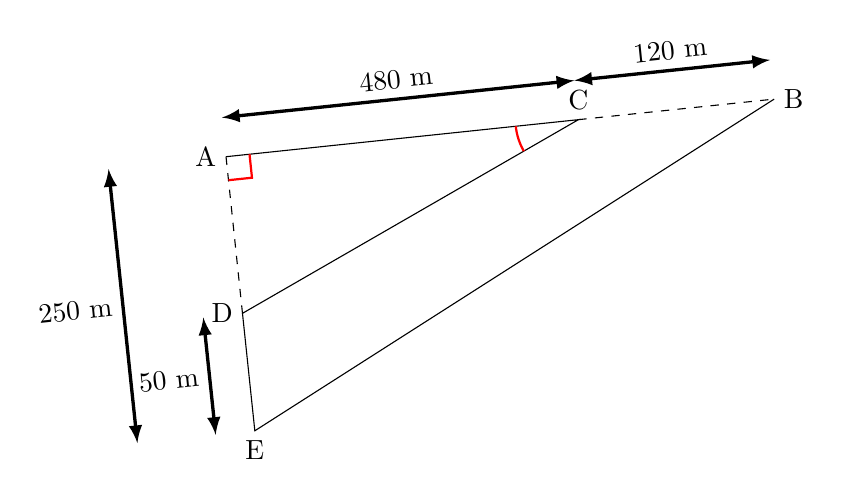
\begin{tikzpicture}[rotate=6,>=latex]
	\coordinate (A) at (0,0);
	\coordinate (B) at (7,0);
	\coordinate (C) at (4.5,0);
	\coordinate (D) at (0,-2);
	\coordinate (E) at (0,-3.5);
	\node[left] at (A) {A};
	\node[right] at (B) {B};
	\node[above] at (C) {C};
	\node[left] at (D) {D};
	\node[below] at (E) {E};
	\draw (A) --(C) -- (D)--(E)--(B);
	\draw[dashed] (A) -- (D)  (C)--(B);
	\draw[line width=1.2pt,<->] (0,0.5) -- (4.5,0.5)
	node[pos=0.5, above, rotate=6]{480 m} ;
	\draw[line width=1.2pt,<->] (4.5,0.5) -- (7,0.5)
	node[pos=0.5, above, rotate=6]{120 m} ;
	\draw[line width=1.2pt,<->] (-0.5,-2) -- (-0.5,-3.5)
	node[pos=0.5, left, rotate=6]{50 m} ;
	\draw[line width=1.2pt,<->] (-1.5,0) -- (-1.5,-3.5)
	node[pos=0.5, left, rotate=6]{250 m} ;
	\draw[red,line width=0.8pt] (0,-0.3) -- (0.3,-0.3) -- (0.3,0) ;
	\draw[red,line width=0.8pt] (3.7,0) arc (180: 204 : 0.8);
	\end{tikzpicture}
	\hfill~

	\begin{enumerate}
		\item Justifier que $\mathrm{AD} = \np[m]{200}$.
		\item Calculer la longueur CD.
		\item Pour que le parcours soit validé il est nécessaire que les droites (CD) et (BE) soient parallèles et que la mesure de l'angle $\widehat{\mathrm{ACD}}$ soit supérieure à $20$\degres.
		\begin{enumerate}
			\item Les droites (CD) et (BE) sont-elles parallèles ?
			\item La mesure de l'angle $\widehat{\mathrm{ACD}}$ est-elle supérieure à $20$\degres ?
			\item Le parcours est-il validé ?
		\end{enumerate}
	\end{enumerate}

\subsection*{Partie B : La natation}

Concernant l'épreuve de natation, il s'agit de nager une distance de \np[m]{200}.

Voici les temps de 9 élèves:\quad5~min~30~s~;~5~min~45~s~;~5~min~49~s~;~5~min~50~s~;~6~min~;~6~min~11~s~;

6~min~12~s~;~6~min~20~s~;~6~min~40.

\begin{enumerate}[resume*]
\item Quel est le temps médian de cette série ?

\item Un poisson rouge nage à la vitesse de \np[km/h]{5}.

Nage-t-il plus vite que l'élève le plus rapide ?
\end{enumerate}

